%%%  کلاس AUTthesis، نسخه آبان 1397
%%%   دانشگاه صنعتی امیرکبیر                 http://www.aut.ac.ir
%%%  تالار گفتگوی پارسی‌لاتک،       http://forum.parsilatex.com
%%%   آپدیت شده در آبان 95
%%%   پشتیبانی و راهنمایی          badali_farhad@yahoo.com
%%%
%%%   بازبینی و اصلاح شده در آبان ماه 1397
%%%  Tested via TeXstudio in TeXlive 2014-2018.
%%%

%-----------------------------------------------------------------------------------------------------
%        روش اجرا.: 2 بار F1 ، 2 بار  F11(به منظور تولید مراجع) ، دوبار Ctrl+Alt+I (به منظور تولید نمایه) و دو بار F1 -------> مشاهده Pdf
%%%%%%%%%%%%%%%%%%%%%%%%%%%%%%%%%%%%%%%%%%%%%%%%%%%%%%
%   TeXstudio as your IDE
%%  برای compile در TeXstudio تنها کافی است منوی Options->Configure TeXstudio را زده و در پنجره Configure TeXstudio در بخش Build گزینه Default Compiler را به XeLaTeX تغییر دهید. سند شما به راحتی compile خواهد شد.
%   F1 & F5 : Build & view
%   F6      : Compile
%   F7      : View
%   --------------
%%%%%%%%%%%%%%%%%%%%%%%%%%%%%%%%%%%%%%%%%%%%%%%%%%%%%%
%        اگر قصد نوشتن رساله دکتری را دارید، در خط زیر به جای msc،
%      کلمه phd را قرار دهید. کلیه تنظیمات لازم، به طور خودکار، اعمال می‌شود.
%%% !TEX TS-program = XeLaTeX
\documentclass[oneside,bsc,12pt]{AUTthesis}
%       فایل commands.tex را حتماً به دقت مطالعه کنید؛ چون دستورات مربوط به فراخوانی بسته زی‌پرشین 
%       و دیگر بسته‌ها و ... در این فایل قرار دارد و بهتر است که با نحوه استفاده از آنها آشنا شوید. توجه شود برای نسخه نهایی پایان‌نامه حتماً hyperref را 
%        غیرفعال کنید.


% در این فایل، دستورها و تنظیمات مورد نیاز، آورده شده است.
%-------------------------------------------------------------------------------------------------------------------
% در ورژن جدید زی‌پرشین برای تایپ متن‌های ریاضی، این سه بسته، حتماً باید فراخوانی شود.
\usepackage{amsthm,amssymb,amsmath,amsfonts}
% بسته‌ای برای تنطیم حاشیه‌های بالا، پایین، چپ و راست صفحه
\usepackage[top=30mm, bottom=30mm, left=25mm, right=30mm]{geometry}
% بسته‌‌ای برای ظاهر شدن شکل‌ها و تصاویر متن
\usepackage{graphicx}
\usepackage{color}
%بسته‌ای برای تنظیم فاصله عمودی خط‌های متن
\usepackage{setspace}
\usepackage{titletoc}
\usepackage{tocloft}
%با فعال کردن بسته زیر فوت‌نوت‌ها در هر صفحه ریست می‌شوند. حالت پیش‌فرض آن ریست شدن در هر فصل می‌باشد.
%\usepackage[perpage]{footmisc}
\usepackage{enumitem}
%\usepackage{titlesec}
% بسته‌ و دستوراتی برای ایجاد لینک‌های رنگی با امکان جهش
\usepackage[pagebackref=false,colorlinks,linkcolor=blue,citecolor=red]{hyperref}
\usepackage[nameinlink]{cleveref}%capitalize,,noabbrev
 \AtBeginDocument{%
    \crefname{equation}{برابری}{equations}%
    \crefname{chapter}{فصل}{chapters}%
    \crefname{section}{بخش}{sections}%
    \crefname{appendix}{پیوست}{appendices}%
    \crefname{enumi}{مورد}{items}%
    \crefname{footnote}{زیرنویس}{footnotes}%
    \crefname{figure}{شکل}{figures}%
    \crefname{table}{جدول}{tables}%
    \crefname{theorem}{قضیه}{theorems}%
    \crefname{lemma}{لم}{lemmas}%
    \crefname{corollary}{نتیجه}{corollaries}%
    \crefname{proposition}{گزاره}{propositions}%
    \crefname{definition}{تعریف}{definitions}%
    \crefname{result}{نتیجه}{results}%
    \crefname{example}{مثال}{examples}%
    \crefname{remark}{نکته}{remarks}%
    \crefname{note}{یادداشت}{notes}%
}
% چنانچه قصد پرینت گرفتن نوشته خود را دارید، خط بالا را غیرفعال و  از دستور زیر استفاده کنید چون در صورت استفاده از دستور زیر‌‌، 
% لینک‌ها به رنگ سیاه ظاهر خواهند شد که برای پرینت گرفتن، مناسب‌تر است
%\usepackage[pagebackref=false]{hyperref}
% بسته‌ لازم برای تنظیم سربرگ‌ها
\usepackage{fancyhdr}
% بسته‌ای برای ظاهر شدن «مراجع»  در فهرست مطالب
\usepackage[nottoc]{tocbibind}
% دستورات مربوط به ایجاد نمایه
\usepackage{makeidx,multicol}
\setlength{\columnsep}{1.5cm}

%%%%%%%%%%%%%%%%%%%%%%%%%%
\usepackage{verbatim}
\makeindex
\usepackage{sectsty}
% فراخوانی بسته زی‌پرشین و تعریف قلم فارسی و انگلیسی
\usepackage{xepersian}%[extrafootnotefeatures]
\SepMark{-}
%حتماً از تک لایو 2014 استفاده کنید.
\settextfont[Scale=1.2]{B Nazanin.ttf}
\setlatintextfont{Times New Roman.ttf}
\renewcommand{\labelitemi}{$\bullet$}
%%%%%%%%%%%%%%%%%%%%%%%%%%
% چنانچه می‌خواهید اعداد در فرمول‌ها، انگلیسی باشد، خط زیر را غیرفعال کنید.
%در غیر اینصورت حتماً فونت PGaramond را نصب کنید.
\setdigitfont[Scale=1.1]{PGaramond.ttf}%%Yas
%%%%%%%%%%%%%%%%%%%%%%%%%%
% تعریف قلم‌های فارسی اضافی برای استفاده در بعضی از قسمت‌های متن
\defpersianfont\nastaliq[Scale=2]{IranNastaliq.ttf}
\defpersianfont\chapternumber[Scale=3]{B Nazanin.ttf}
%\chapterfont{\centering}%
%%%%%%%%%%%%%%%%%%%%%%%%%%
% دستوری برای تغییر نام کلمه «اثبات» به «برهان»
\renewcommand\proofname{\textbf{برهان}}

% دستوری برای تغییر نام کلمه «کتاب‌نامه» به «منابع و مراجع«
\renewcommand{\bibname}{منابع و مراجع}


% Headings for every page of ToC, LoF and Lot
\setlength{\cftbeforetoctitleskip}{-1.2em}
\setlength{\cftbeforelottitleskip}{-1.2em}
\setlength{\cftbeforeloftitleskip}{-1.2em}
\setlength{\cftaftertoctitleskip}{-1em}
\setlength{\cftafterlottitleskip}{-1em}
\setlength{\cftafterloftitleskip}{-1em}
%%\makeatletter
%%%%\renewcommand{\l@chapter}{\@dottedtocline{1}{1em\bfseries}{1em}}
%%%%\renewcommand{\l@section}{\@dottedtocline{2}{2em}{2em}}
%%%%\renewcommand{\l@subsection}{\@dottedtocline{3}{3em}{3em}}
%%%%\renewcommand{\l@subsubsection}{\@dottedtocline{4}{4em}{4em}}
%%%%\makeatother


\newcommand\tocheading{\par عنوان\hfill صفحه \par}
\newcommand\lofheading{\hspace*{.5cm}\figurename\hfill صفحه \par}
\newcommand\lotheading{\hspace*{.5cm}\tablename\hfill صفحه \par}

\renewcommand{\cftchapleader}{\cftdotfill{\cftdotsep}}
\renewcommand{\cfttoctitlefont}{\hspace*{\fill}\LARGE\bfseries}%\Large
\renewcommand{\cftaftertoctitle}{\hspace*{\fill}}
\renewcommand{\cftlottitlefont}{\hspace*{\fill}\LARGE\bfseries}%\Large
\renewcommand{\cftafterlottitle}{\hspace*{\fill}}
\renewcommand{\cftloftitlefont}{\hspace*{\fill}\LARGE\bfseries}
\renewcommand{\cftafterloftitle}{\hspace*{\fill}}

%%%%%%%%%%%%%%%%%%%%%%%%%%
% تعریف و نحوه ظاهر شدن عنوان قضیه‌ها، تعریف‌ها، مثال‌ها و ...
%برای شماره گذاری سه تایی قضیه ها
\theoremstyle{definition}
\newtheorem{definition}{تعریف}[section]
\newtheorem{remark}[definition]{نکته}
\newtheorem{note}[definition]{یادداشت}
\newtheorem{example}[definition]{نمونه}
\newtheorem{question}[definition]{سوال}
\newtheorem{remember}[definition]{یاداوری}
\theoremstyle{theorem}
\newtheorem{theorem}[definition]{قضیه}
\newtheorem{lemma}[definition]{لم}
\newtheorem{proposition}[definition]{گزاره}
\newtheorem{corollary}[definition]{نتیجه}
%%%%%%%%%%%%%%%%%%%%%%%%
%%%%%%%%%%%%%%%%%%%
%%% برای شماره گذاری چهارتایی قضیه ها و ...
%%\newtheorem{definition1}[subsubsection]{تعریف}
%%\newtheorem{theorem1}[subsubsection]{قضیه}
%%\newtheorem{lemma1}[subsubsection]{لم}
%%\newtheorem{proposition1}[subsubsection]{گزاره}
%%\newtheorem{corollary1}[subsubsection]{نتیجه}
%%\newtheorem{remark1}[subsubsection]{نکته}
%%\newtheorem{example1}[subsubsection]{مثال}
%%\newtheorem{question1}[subsubsection]{سوال}

%%%%%%%%%%%%%%%%%%%%%%%%%%%%

% دستورهایی برای سفارشی کردن صفحات اول فصل‌ها
\makeatletter
\newcommand\mycustomraggedright{%
 \if@RTL\raggedleft%
 \else\raggedright%
 \fi}
\def\@makechapterhead#1{%
\thispagestyle{style1}
\vspace*{20\p@}%
{\parindent \z@ \mycustomraggedright
\ifnum \c@secnumdepth >\m@ne
\if@mainmatter

\bfseries{\Huge \@chapapp}\small\space {\chapternumber\thechapter}
\par\nobreak
\vskip 0\p@
\fi
\fi
\interlinepenalty\@M 
\Huge \bfseries #1\par\nobreak
\vskip 120\p@

}

%\thispagestyle{empty}
\newpage}
\bidi@patchcmd{\@makechapterhead}{\thechapter}{\tartibi{chapter}}{}{}
\bidi@patchcmd{\chaptermark}{\thechapter}{\tartibi{chapter}}{}{}
\makeatother

\pagestyle{fancy}
\renewcommand{\chaptermark}[1]{\markboth{\chaptername~\tartibi{chapter}: #1}{}}

\fancypagestyle{style1}{
\fancyhf{} 
\fancyfoot[c]{\thepage}
\fancyhead[R]{\leftmark}%
\renewcommand{\headrulewidth}{1.2pt}
}


\fancypagestyle{style2}{
\fancyhf{}
\fancyhead[R]{چکیده}
\fancyfoot[C]{\thepage{}}
\renewcommand{\headrulewidth}{1.2pt}
}

\fancypagestyle{style3}{%
  \fancyhf{}%
  \fancyhead[R]{فهرست نمادها}
  \fancyfoot[C]{\thepage}%
  \renewcommand{\headrulewidth}{1.2pt}%
}

\fancypagestyle{style4}{%
  \fancyhf{}%
  \fancyhead[R]{فهرست جداول}
  \fancyfoot[C]{\thepage}%
  \renewcommand{\headrulewidth}{1.2pt}%
}

\fancypagestyle{style5}{%
  \fancyhf{}%
  \fancyhead[R]{فهرست اشکال}
  \fancyfoot[C]{\thepage}%
  \renewcommand{\headrulewidth}{1.2pt}%
}

\fancypagestyle{style6}{%
  \fancyhf{}%
  \fancyhead[R]{فهرست مطالب}
  \fancyfoot[C]{\thepage}%
  \renewcommand{\headrulewidth}{1.2pt}%
}

\fancypagestyle{style7}{%
  \fancyhf{}%
  \fancyhead[R]{نمایه}
  \fancyfoot[C]{\thepage}%
  \renewcommand{\headrulewidth}{1.2pt}%
}

\fancypagestyle{style8}{%
  \fancyhf{}%
  \fancyhead[R]{منابع و مراجع}
  \fancyfoot[C]{\thepage}%
  \renewcommand{\headrulewidth}{1.2pt}%
}
\fancypagestyle{style9}{%
  \fancyhf{}%
  \fancyhead[R]{واژه‌نامه‌ی فارسی به انگلیسی}
  \fancyfoot[C]{\thepage}%
  \renewcommand{\headrulewidth}{1.2pt}%
}
%


%دستور حذف نام لیست تصاویر و لیست جداول از فهرست مطالب
\newcommand*{\BeginNoToc}{%
  \addtocontents{toc}{%
    \edef\protect\SavedTocDepth{\protect\the\protect\value{tocdepth}}%
  }%
  \addtocontents{toc}{%
    \protect\setcounter{tocdepth}{-10}%
  }%
}
\newcommand*{\EndNoToc}{%
  \addtocontents{toc}{%
    \protect\setcounter{tocdepth}{\protect\SavedTocDepth}%
  }%
}
\newcounter{savepage}
\renewcommand{\listfigurename}{فهرست اشکال}
\renewcommand{\listtablename}{فهرست جداول}
%\renewcommand\cftsecleader{\cftdotfill{\cftdotsep}}
%%%%%%%%%%%%%%%%%%%%%%%%%%%%%
%%%%%%%%%%%%%%%%%%%%%%%%%%%%

\begin{document}
\baselineskip=.75cm
\linespread{1.75}
%% -!TEX root = AUTthesis.tex
% در این فایل، عنوان پایان‌نامه، مشخصات خود، متن تقدیمی‌، ستایش، سپاس‌گزاری و چکیده پایان‌نامه را به فارسی، وارد کنید.
% توجه داشته باشید که جدول حاوی مشخصات پروژه/پایان‌نامه/رساله و همچنین، مشخصات داخل آن، به طور خودکار، درج می‌شود.
%%%%%%%%%%%%%%%%%%%%%%%%%%%%%%%%%%%%
% دانشکده، آموزشکده و یا پژوهشکده  خود را وارد کنید
\faculty{دانشکده مهندسی کامپیوتر}

% عنوان پایان‌نامه را وارد کنید
\fatitle{بررسی چالش های پیاده سازی\lr{edge computing } و تاثیرات آن  بر تکلونوژی
\\[.75 cm]
 پایان‌نامه}
% نام استاد(ان) راهنما را وارد کنید
\firstsupervisor{دکتر صفابخش}
%\secondsupervisor{استاد راهنمای دوم}
% نام استاد(دان) مشاور را وارد کنید. چنانچه استاد مشاور ندارید، دستور پایین را غیرفعال کنید.
\firstadvisor{دکتر صفابخش}
%\secondadvisor{استاد مشاور دوم}
% نام نویسنده را وارد کنید
\name{محمد }
% نام خانوادگی نویسنده را وارد کنید
\surname{اژدری}
%%%%%%%%%%%%%%%%%%%%%%%%%%%%%%%%%%
\thesisdate{فروردین ۹۸}

% چکیده پایان‌نامه را وارد کنید
\fa-abstract{
در اين قسمت چكيده پایان نامه نوشته مي‌شو‌د‌.‌ چكيده بايد جامع و بيان‌كننده‌ خلاصه‌اي از اقدامات انجام‌شده باشد. در چكيده باید از ارجاع به مرجع و ذكر روابط رياضي، بيان تاريخچه و تعريف مسئله خودداري ‌شود. 
}


% کلمات کلیدی پایان‌نامه را وارد کنید
\keywords{کلیدواژه اول، ...، کلیدواژه پنجم (نوشتن سه تا پنج واژه کلیدی ضروری است)}



\AUTtitle
%%%%%%%%%%%%%%%%%%%%%%%%%%%%%%%%%%
\vspace*{7cm}
\thispagestyle{empty}
\begin{center}

\includegraphics[height=5cm,width=12cm]{besm}
\end{center}
% تاییدیه دفاع
\newpage
\thispagestyle{empty}
%\fontsize{18pt}{19pt}\selectfont

\section*{صفحه فرم ارزیابی و تصویب پایان نامه- فرم تأیید اعضاء كميته دفاع}

\fontsize{12pt}{14pt}\selectfont
%\renewcommand{\baselinestretch}{1.5}
\vspace*{1cm}
   در این صفحه فرم دفاع یا تایید و تصویب پایان نامه موسوم به فرم کمیته دفاع- موجود در پرونده آموزشی- را قرار دهید.
\vspace*{1cm}


\subsection*{نکات مهم:}
 
\begin{itemize}
\item
	نگارش پایان نامه/رساله باید به
	{\color{red}
		زبان فارسی
	}
	و بر اساس آخرین نسخه دستورالعمل و راهنمای تدوین پایان نامه های دانشگاه صنعتی امیرکبیر باشد.(دستورالعمل و راهنمای حاضر)
\item رنگ جلد پایان نامه/رساله چاپي كارشناسي، كارشناسي ارشد و دكترا  بايد به ترتيب مشكي، طوسي و سفيد رنگ باشد.  
\item چاپ و صحافی پایان نامه/رساله بصورت
{\color{red}
	پشت و رو(دورو)
}
بلامانع است و انجام آن توصيه مي شود. 
\end{itemize}
%%%%%%%%%%%%%%%%%%%%%%%%%%%%%%%%%%%%%%%%%%%%%%%%%%%%%%%%%%%%%%%%%%%%%%%%%%%%%%%%%%%%%%%%%%%%%%%%%%
%%%%%%%%%%%%%%%%%%%%%%%%%%%%%%%%%%%%%%%%%%%%%%%%%%%%%%%%%%%%%%%%%%%%%%%%%%%%%%%%%%%%%%%%%%%%%%%%%%
\newpage
\thispagestyle{empty}
\begin{picture}(50,50)
  \put(17,0){
\includegraphics[scale=1.1]{fa-logo}}
  \put(4.5,-13){\footnotesize{دانشگاه صنعتی امیرکبیر}}
  \put(10.5,-27){\footnotesize{(پلی‌تکنیک تهران)}}
  \put(170,30){\bf{به نام خدا}}
  \put(140,-5){\Large\bf{تعهدنامه اصالت اثر}}
  \put(310,0){تاریخ: \datethesis}
\end{picture}

\vspace*{2.5cm}

اينجانب {\bf{\fname\lname}} متعهد می‌شوم که مطالب مندرج در این پایان‌نامه حاصل کار پژوهشی اینجانب تحت نظارت و راهنمایی اساتید دانشگاه صنعتی امیرکبیر بوده و به دستاوردهای دیگران که در این پژوهش از آنها استفاده شده است مطابق مقررات و روال متعارف ارجاع و در فهرست منابع و مآخذ ذکر گردیده است. این پایان‌نامه قبلاً برای احراز هیچ مدرک هم‌سطح یا بالاتر ارائه نگردیده است.

در صورت اثبات تخلف در هر زمان، مدرک تحصیلی صادر شده توسط دانشگاه از درجه اعتبار ساقط بوده و دانشگاه حق پیگیری قانونی خواهد داشت.


کلیه نتایج و حقوق حاصل از این پایان‌نامه متعلق به دانشگاه صنعتی امیرکبیر می‌باشد. هرگونه استفاده از نتایج علمی و عملی، واگذاری اطلاعات به دیگران یا چاپ و تکثیر، نسخه‌برداری، ترجمه و اقتباس از این پایان نامه بدون موافقت کتبی دانشگاه صنعتی امیرکبیر ممنوع است. 
نقل مطالب با ذکر مآخذ بلامانع است.\\
\vspace{2.5cm}


{\centerline {\bf{\fname\lname}}}
\vspace*{.2cm}
{\centerline{امضا}}
%%%%%%%%%%%%%%%%%%%%%%%%%%%%%%%%%
% چنانچه مایل به چاپ صفحات «تقدیم»، «نیایش» و «سپاس‌گزاری» در خروجی نیستید، خط‌های زیر را با گذاشتن ٪  در ابتدای آنها غیرفعال کنید.
% پایان‌نامه خود را تقدیم کنید
% نیایش خود را در فایل زیر بنویسید.
\begin{acknowledgementpage}

\vspace{1.5cm}

{\nastaliq
{
تقدیم به همه دوستانم که در راه پیشرفت زندگیم نکته‌های بسیاری را به من یاد دادند.
}}\end{acknowledgementpage}
\newpage
% سپاسگزاری را در فایل زیر بنویسید.
%%%%%%%%%%%%%%%%%%%%%%%%%%%%%%%%%%%%
\newpage\thispagestyle{empty}
% سپاس‌گزاری
{\nastaliq
سپاس‌گزاری
}
\\[2cm]

بدین وسیله تقدیر و تشکر میکنم از دکتر صفابخش که استاد راهنمای بنده و آموزنده روش‌های اصولی پژوهش و تحقیق برای بنده بودند.











% با استفاده از دستور زیر، امضای شما، به طور خودکار، درج می‌شود.
\signature








%%%%%%%%%%%%%%%%%%%%%%%%%%%%%%%%%%%%%%%%%
%%%%%%%%%%%%%%%%%%%%%%%%%%%%%%%%%کدهای زیر را تغییر ندهید.
\newpage\clearpage

\pagestyle{style2}

\vspace*{-1cm}
\section*{\centering چکیده}
%\addcontentsline{toc}{chapter}{چکیده}
\vspace*{.5cm}
\ffa-abstract
\vspace*{2cm}


{\noindent\large\textbf{واژه‌های کلیدی:}}\par
\vspace*{.5cm}
\fkeywords
% دستور زیر برای شماره گذاری صفحات قبل از فصل اول با حروف ابجد است.
\pagenumbering{alph}
%-----------------------------------------------------------------------------
% فایل زیر دستورات مربوط به نمایش صفحات فهرست مطالب- فهرست اشکال و جداول است.
%{\pagestyle{style2}
%\tableofcontents}\newpage
%
%\listoffigures
\cleardoublepage
\pagestyle{style6}
\tableofcontents
\pagestyle{style6}
\cleardoublepage
%اگر لیست تصاویر و لیست جداول ندارید ، کدهای زیر را با گذاشتن % در ابتدای آنها، غیرفعال کنید.
\BeginNoToc
%============
\addtocontents{lof}{\lofheading}% add heading to the first page in LoF
\pagestyle{style5}
\listoffigures
\thispagestyle{style5}
\cleardoublepage
%============
\addtocontents{lot}{\lotheading}% add heading to the first page in LoT
\thispagestyle{style4}
\listoftables
\thispagestyle{style4}
%============
%\cleardoublepage
%
\cleardoublepage
\setcounter{savepage}{\arabic{page}}
\mainmatter
\addtocontents{toc}{\tocheading}% add heading to the first page in ToC, after frontmatter entries
\EndNoToc
% در صورت تمایل می‌توانید با فعال کردن دستور بالا، لیست تصاویر را به  پایان‌نامه خود اضافه کنید.
%-------------------------------------------------------------------------symbols(فهرست نمادها)
% وجود لیست نمادها الزامیست.(لطفاً نمادهای خود را جایگذین نمادهای پیش‌فرض کنید.)
%%%%%%%%%%%%%

{\centering\LARGE\textbf{فهرست نمادها}\par}%

\pagenumbering{alph}
\setcounter{page}{\thesavepage}
%\setcounter{page}{6}
\vspace*{1cm}

\pagestyle{style3}
%\thispagestyle{empty}
%\addcontentsline{toc}{chapter}{فهرست نمادها}
\symb{\text{ نماد}}{مفهوم}
\\
%مقادیر بالا را تغییر ندهید
%%%%%%%%%%%%%%%%%%%%%%%%%%%%%%%%%%%%%%%%%%%%%%%%%%%%%%%%%

%%%%%%%%%%%%%%%%%%%%%%%%%%%%%%%%%%%%%%%

\thispagestyle{style3}
\newpage
%\pagestyle{style1}
%%%%%%%%%%%%%%%%%%%%%%%%%%%%%%%%%%%%


\pagenumbering{arabic}
\pagestyle{style1}
%--------------------------------------------------------------------------chapters(فصل ها)
\chapter{معرفی و مقدمات \lr{edge computing } }

\section{مقدمه}
با توجه به پیشرفت روزافزون تکلونوژی شبکه و اینترنت اشیا و همچنین نیازهایی که به این حوزه به وجود می‌آید، بازار خیلی بزرگی در دنیا برای این صنعت به وجود آمده است.

از این رو شرکت‌های زیادی به منظور سرویس‌دهی بر پایه اینترنت اشیا به وجود آمده‌اند و در حال پیاده‌سازی برنامه‌ها و دستگاه‌های مختلف، چه در قسمت نرم‌افزار و چه در قسمت سخت‌افزار هستند.

در پیاده‌سازی یک پلتفرم اینترنت اشیا، چالش‌های مختلفی وجود دارد.
در میان این‌ها، مسئله حجم بزرگ داده‌ها و محاسبات سنگینی که روی آن‌ها انجام می‌گیرد، یکی از چالش‌های عمده‌ی این کار است.

که در این تحقیق به این چالش و یکی از روش‌های حل آن که \lr{edge computing } است، می‌پردازیم.


\section{محاسبات زیاد، چرا، کجا و چگونه!؟}\label{sec2}
ابتدا کمی درمورد اینترنت اشیا سخن می‌گوییم. اگر بخواهیم به صورت ساده به معرفی این حوزه بپردازیم میتوانیم بگوییم که ارتباط اجزای سخت‌افزاری مختلف مانند  \lr{gadget}های گوناگون تا کارهای بزرگ مانند نیروگاه‌های برق، از طریق اینترنت با هم.

برای مثال فرض کنید یخچال شما آن‌قدر هوشمند است که اگر تخم‌مرغ تمام شد، یا کم مانده بود متوجه میشود و به صورت آنلاین سفارش میدهد و برایتان تخم‌مرغ می‌خرد.
یا یک مثال بزرگ‌تر که یک نیروگاه برق متوجه میشود که در لحظه چقدر برق نیاز است که تولید کند.

همه این‌ها از کوچک به بزرگ دنیای اینترنت اشیا را تشکیل می‌دهند که در دنیای مدرن امروز،‌ روزبه‌روز با پیشرفت همراه است. و نیازش بیشتر احساس می‌شود.
اما همان‌طور که گفتیم، برای پیاده‌سازی این صنعت چالش‌های مختلفی وجود دارد که حجم بزرگ داده‌ها و محاسبات زیاد از اساسی‌ترین آن‌ها به شمار می‌رود.

حالا چرا داده‌ها زیاد هستند؟ دلیلش کمی بارز است. یک شهر هوشمند را تصور کنید که میخواهد حتی خالی بودن سطل آشغال‌های پارک‌هایش را متوجه بشود که مامورهای شهرداری برای خالی کردن آن‌ها اقدام کنند . چراغ راهنمایی‌هایی هوشمندی میخواهد که از ترافیک کل شهر اطلاع داشته باشند و بر اساس آن‌ها عمل کنند.

همه این‌ها نیازمند پردازش و انتقال اطلاعات زیادی است.
حالا این اطلاعات کجا ذخیره می‌شوند و کجا پردازش؟
قاعدتا یک چراغ راهنما آن‌قدر حافظه برای این اطلاعات ندارد و باید از طریق شبکه اینترنت به فضای ابری پلتفرم اصلی وصل شود و به صورت مرتب با آن اطلاعات رد و بدل کند.
بدیهی است که بسیاری از محاسبات را می‌توانیم در همان فضای ابری انجام دهیم و دیگر نیازی نباشد که خود\lr{gadget}  پردازشی انجام بدهد.

خب تا اینجا همه چیز حل شده است و چالشی احساس نمی‌شود!

\section{چالش اصلی کجاست؟}
در برخی از حالت‌ها و دستگاه‌ها آن‌قدر سرعت پردازش و حتی امنیت و قابل اعتماد بودن آن مطرح هست که در مسئله‌ی اینکه این پردازش‌ها کجا انجام پذیرد مسئله مهمی به شمار می‌رود.
برای مثال یک ماشین هوشمند را نظر بگیرید، که واقعا نیاز دارد کاملا اطلاعاتش سربع و دقیق پرداش شوند. حالا اگر این پردازش‌ها در فضای ابری انجام شوند و از طریق اینترنت انجام شوند، ممکن است خطاهایی رخ بدهد و باعث آسیب‌های جبران ناپذیری بشود.

اینجاست که مفهوم \lr{edge computing} مطرح میشود که بیانگر این است که این محاسبات یا در همان خود دستگاه و یا در جایی که هیچ خطای چه شبکه و چه کمبود منابع رخ بدهد، انجام بشوند.
چه در خود دستگاه و چه در جایی نزدیک آن.

\section{برخی مواردی که \lr{edge computing} اهمیت پیدا میکند.}
\subsection{حمل و نقل هوشمند}
ماشین‌های هوشمند را درواقع میتوان کامپیوترهای خیلی هوشمند متحرک درنظر گرفت.
در این ماشین‌هانمی‌توان پردازش‌ها را در فضای ابری انجام داد، زیرا مسیر رفت و برگشت هم کند است و خطاهای زیادی دارد و یک ماشین نمی‌تواند منتظر پاسخ چیزی باشد تا براساس آن تصمیم بگیرد.
در اینجا همه محاسبات باید در نزدیک ترین جای ممکن به سنسورها انجام شده و در سریع‌ترین زمان ممکن بدون خطای انتقال به آن‌ها برسد.
\subsection{حوزه سلامت و پزشکی}
همان‌طور که قبلا هم اشاره شد، اینترنت اشیا در حوزه‌های بسیاری ورود کرده که پزشکی هم از این قاعده مستثنی نیست.
و اتقافا بازارهای بزرگ اینترنت اشیا حساب می‌شود.

حالا اینجا هم ممکن است محاسبات در \lr{cloud}  انجام شوند و ممکن است در نزدیک‌ترین جا به سنسور.
مثلا در سنسورهایی که داخل دستگاه‌های جراحی قرار دارند و یا بعضی از ساعت‌های هوشمند که اطلاعات سلامت افراد را جمع آوری میکنند، پردازش‌ها در لبه سنسور انجام می‌شوند. و نیازی نیست با فضای ابری اطلاعاتی در لحظه رو و بدل شود.
\subsection{کشاورزی}
با توجه به موقعیت مکانی دوردست مزارع ، که بسیاری از آنها دسترسی محدود به پهنای باند دارند، کشاورزی یک نامزد اصلی برای بهره مندی از \lr{edge computing} است. برخلاف ماهواره های تمام وقت یا اتصالات مایکروویو، \lr{edge computing}  گزینه ای پایدار و مقرون به صرفه را ارائه می دهد. مزارع هوشمند می توانند از اینترنت اشیا برای ردیابی مکان تجهیزات ، دمای محیط و عملکرد تجهیزات استفاده کنند.

\subsection{خرده‌فروشی}
آینده سوپر مارکت شامل \textbf{قفسه های هوشمند} با کمک اینترنت اشیا خواهد بود. با استفاده از سنسورهای \lr{RFID (ID Radio Frequency) } در قفسه ها ، شرکت های خرده فروشی قادر به جمع آوری داده ها هستند. در بعضی موارد ، روبات ها قفسه‌ها را اسکن می کنند تا به دنبال مواردی باشند که نیاز به راه اندازی مجدد دارند. برخی از فروشگاه‌های خرده‌فروشی حتی به میهمانان اجازه می دهند با وسایل خود از فروشگاه خارج شوند و کارت های خود را از طریق یک برنامه موبایل شارژ کنند. این امر باعث می شود زمان انتظار برای رونق گرفتن و یک تجربه خرید بدون درز برای مهمانان کاهش یابد.
\subsection{انرژی}
برای شرکت های نفت و گاز و انرژی، \lr{edge computing} می‌تواند تولید، فرآیندها و امنیت را بهبود بخشد.به وفور در بسیاری از مناطق دور افتاده، شرکت های انرژی برای پردازش اطلاعات به اندازه کافی سریع برای رفع نیازهای خود بدون اتصال به فضای ابری، تلاش می کنند. سنسورهایی را در نظر بگیرید که پمپ های نفتی را در این زمینه رصد می کنند که امروز باید از نزدیک با نظارت انسانی کنترل شوند. پردازش داده های زمان واقعی باعث می شود شرکت های انرژی برای هشدار نسبت به مشکلات این پمپ های نفتی به منظور جلوگیری از نظارت غیر ضروری بر هزینه های سربار و بهبود زمان پاسخ دادن به مسئله هشدار دهند.

\chapter{پیشرفت و توسعه‌ی \lr{edge computing} در صنعت}

\section{بررسی \lr{intelligent edge computing}}
تا اینجا با مفهوم، چرایی و برخی کاربردهای \lr{edge computing} آشنا شده‌ایم.
با بررسی‌ها و پیشرفت‌هایی که در این حوزه انجام شده، مشخص شده است که انتخاب اینکه محاسبات در حالت‌های مختلف در کجا باید انجام بگیرد تا بهترین خروجی حاصل گردد، امری مهم است.
حالا چند معقوله مطرح می‌شود، یکی اینکه به صورت پیش‌فرض این حالت در دستگاه باشد که محاسبات را در جای به‌خصوصی انجام دهد.
ولی حالت بعدی پا را فراتر از این می‌گذارد و از هوشمند سازی سنسور یا دستگاه در انتخاب این موضوع صحبت میکند که در آن دستگاه از تکلونوژی‌های یادگیری ماشین و یادگیری عمیق بهره می‌برد که این تصمیم را در بهترین وجه بگیرد.

در این فصل به بررسی اجمالی معماری اینترنت اشیای یک شهر هوشمند می‌پردازیم و نقش \lr{intelligent edge computing} را در آن بررسی می‌کنیم.

\section{بررسی معماری مدیریت انرژی بر پایه اینترنت اشیای یک شهر هوشمند\cite{liu2019intelligent}}
\subsection{ساختمان‌های هوشمند}
اگر بخواهیم یک شهر هوشمند داشته باشیم، قاعدتا باید از ساختمان‌های هوشمند شروع کنیم.
ساختمانی را تصور کنید که همه چیز در آن تحت کنترل است و به صورت خودکار انجام میشود. مثلا: با زیاد شدن دمای هوا، کولر روشن می‌شود و با کم شدنش خاموش می‌شود.

حالا اگر بخواهیم این ساختمان را از نظر انرژی بررسی کنیم در سه سطح قابل بررسی است:


\begin{enumerate}
    \item سطح دستگاه\footnote{\lr{Device Level}}
    \item سطح سیسنم\footnote{\lr{System Level}}
    \item سطح بین سیستم\footnote{\lr{Inter-System Level}}
\end{enumerate}

سطح دستگاه:

دستگاه های موجود در ساختمان های هوشمند می توانند دسترسی به داده های ورودی (برق مصرفی ، دما ، رطوبت و غیره) را که مربوط به آگاهی موقعیتی در مورد شرایط عملیاتی آن است، گسترش دهند. به طور خاص، برای مدیریت انرژی، واحد پردازش \lr{IOT} باید داده های انرژی را به صورت پیش بینی یا تطبیقی پردازش کند و خروجی را به واحدهای فرماندهی و کنترل مربوط منتقل کند. سپس محرک های نهایی می توانند اقدامات لازم را انجام دهند.


سطح سیستم:

در سطح سیستم، عملکرد اصلی یک ساختمان هوشمند، هماهنگی و هماهنگ سازی رفتارهای مؤلفه های مختلف مرتبط با انرژی است. برای مدیریت بهتر و کنترل واحدهای مرتبط با انرژی، ساختمان هوشمند می تواند به طور خودکار سیستم اصلی داخلی ساختمان مورد حمایت سیستم \lr{IOT}را در کوتاه مدت تنظیم کند. برنامه های مرتبط با انرژی همچنین توسط بسیاری از دستگاه های هوشمند \lr{IOT} مستقر در سیستم پشتیبانی می شوند.


سطح بین سیستم:

به ادغام چندین زیر سیستم مستقل اشاره دارد و به منظور دستیابی به مدیریت انرژی برای ساختمان‌های هوشمند، در کنار هم کار می کنند. به این معنا ،یک ساختمان هوشمند یک سیستم بین شهری است که در آن برق ، گاز، گرمایش و سایر سیستم ها به عنوان یک سیستم واحد یکپارچه می شوند. هوشمندی آن حاکی از ظرفیت مدیریت، اتصال، و تطبیق دارایی ها و کارکردهای مختلف (از جمله عوامل فنی، اقتصادی و اجتماعی) برای رضایت از مدیریت انرژی است.


\subsection{شبکه برق هوشمند}
شبکه برق هوشمند یکی از مؤلفه های اصلی استراتژی های مربوط به آینده انرژی پایدار است. با استفاده از \lr{IOT}، آنها نه تنها می توانند 112 منابع انرژی تجدیدپذیر و الکترودسازی حمل و نقل را تسهیل کنند، بلکه خدمات جدیدی با ارزش افزوده مرتبط با انرژی ارائه دهند.

به طور خاص، تغییر مدیریت انرژی با طراحی و استقرار شبکه های هوشمند هدایت می شود. شبکه های برق هوشمند قابلیت گسترش قابلیت های خود را با هوشمندی و جریان داده ها دارند. با کمک \lr{IOT}، مدیریت انرژی در شبکه های برق هوشمند می تواند به هر گوشه از شهر برسد و زیرساخت های شبکه هوشمند و تعامل کاربر پسند را تحریک می‌کند.
انرژی هوشمند به همراه اینترنت توسعه جدید سیستم های مدیریت نیرو با تلفیق عمیق اینترنت و تولید انرژی، انتقال، ذخیره سازی، مصرف و بازار است.

ویژگی های اصلی آن شامل هوشمند بودن تجهیزات، چندین نوع انرژی همزمان، اطلاعات متقارن، تقاضا و تقاضا توزیع می شود، سیستم مسطح و معاملات باز است. به عنوان مثال توسعه امکانات تولید و مصرف انرژی هوشمند از جمله معادن ذغال سنگ هوشمند، مزارع بادی هوشمند، ایستگاه های \lr{PV} هوشمند و غیره و همچنین سکوهای ابری با بهره برداری هوشمند مبتنی بر اینترنت، به منظور تحقق بهینه سازی کنترل از راه دور و بهبود کارایی بهره برداری و سود.


\subsection{شبکه‌های چندتایی}
شبکه های چندتایی مبتنی بر \lr{IOT} می توانند بهره وری کلی و بهره مندی از سیستم انرژی را در مناطق با اندازه های مختلف از جمله ساختمان های بزرگ، پارک ها، جزایر، شهرها و ... بهبود بخشند.

بر اساس تکلونوژی مورد استفاده در سیستم \lr{IOT}، شبکه های چند انرژی می توانند شبکه الکتریکی هوشمند، شبکه های گرما و گاز و ترافیک شبکه را برای مدیریت یکپارچه انرژی برای شهرهای هوشمند ادغام کنند. علاوه بر این، مزایای استفاده از \lr{IOT} در یک سیستم چند انرژی در زیر ذکر شده است.


\begin{enumerate}
    \item ترویج ادغام عمیق زیرساخت‌های انرژی و اطلاعات
    
    \begin{itemize}
        \item براساس فن آوری \lr{IOT}، یک سیستم چند انرژی می تواند ساخت شبکه های انرژی از جمله برق، گاز، هوای خنک، گرما و ... را با زیرساخت های اطلاعاتی خود از جمله معماری اطلاعات، واحد ذخیره سازی و غیره هماهنگ کند. بدین ترتیب، سیستم اطلاعاتی و سیستم انرژی، در اندازه گیری، محاسبه، کنترل و غیره می توانند بسیار کارآمد شوند. این ادغام می تواند ساختار استاندارد شبکه و انرژی و رابط اطلاعاتی را ایجاد کند.
    \end{itemize}
    
    \item توسعه مدیریت هوشمند انرژی
    \begin{itemize}
        \item از طریق توسعه شبکه های \lr{IOT} پیشرفته، امکانات نهایی از جمله خانه های هوشمند، مناطق هوشمند و غیره می توانند بسترهای نظارت بر کارآیی انرژی را بسازند، خدمات مدیریت انرژی و صرفه جویی در مصرف انرژی را ارائه دهند و به شخصی سازی هوشمند و معاملات انعطاف پذیر انرژی پی ببرند.
        
    \end{itemize}
    \item پرورش و استفاده از بازار انرژی‌های جدید
    \begin{itemize}
        \item با استفاده از یک سیستم اینترنت اشیا، اشخاص چند انرژی می توانند به جمع آوری اتوماتیک از راه دور و خواندن آب، گاز، گرما و برق در یک کنتور مشترک برسند. این مزیت یک سیستم انرژی مبتنی بر اینترنت اشیا می تواند یک سیستم بازار آزاد و مشترک را شامل شود که شامل کاربران کوچک و خرد مانند افراد، خانواده ها و منابع انرژی توزیع شده برای به اشتراک گذاری و تجارت انرژی با انعطاف پذیری و مساوی از طریق سیستم عامل های یکپارچه می شود.
    \end{itemize}
    
\end{enumerate}

\begin{figure}[!h]
\centerline{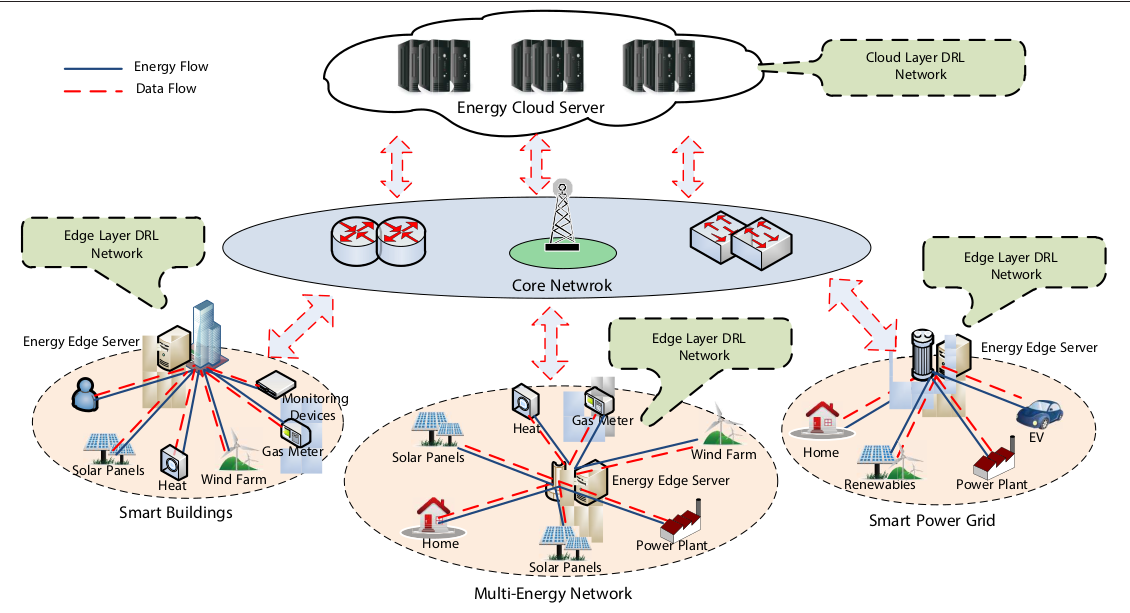
\includegraphics[width=.85\textwidth]{f-2-1.png}}
\caption{معماری کلی مدیریت انرژی یک شهر هوشمند بر پایه اینترنت اشیا}
\end{figure}

\chapter{نگارش صحيح}
%\thispagestyle{empty}

\section{مقدمه}

فصل مقدمه یک پایان نامه، با بیان نیاز موضوع، تعريف مسئله و اهمیت آن در یک یا چند بند (پاراگراف) آغاز مي‌شود\footnote{شروع مقدمه نبايد چنان طولاني باشد كه هدف اصلي را تحت‌ تاثير قرار دهد.}  و با مرور پيشينه موضوع (سابقه کارهای انجام‌شده پیشین که ارتباط مستقیمی با مسئله مورد بررسی دارند) ادامه مي‌يابد. سپس در یک یا دو بند توضیح داده مي‌شود كه در این پایان نامه، چه ديدگاه يا راهكار جدیدي نسبت به مسئله (موضوع) مورد بررسي وجود دارد. به‌عبارت دیگر نوآوری‌ها به‌صورت کاملاً شفاف و صریح بیان می‌شود. در ادامه ممکن است به نتايج بدست‌آمده نیز به‌طور مختصر و کلی اشاره ‌شود. در آخرین بند از مقدمه به محتواي فصل‌هاي بعدي پایان نامه به‌اختصار اشاره مي‌شود.\\
برای مشاهده دستورالعمل کامل دانشگاه صنعتی امیرکبیر(پلی تکنیک تهران) به \cite{zakeri} یا به سایت
%
\href{http://library.aut.ac.ir/Thesis%20Guide}{کتابخانه دانشگاه صنعتی امیرکبیر(پلی تکنیک تهران)}%
مراجعه نمایید.

نگارش صحيح يک پایان نامه در فهم آسان آن بسيار موثر است. در اين فصل مهمترین قواعد نگارشی که باید مورد توجه جدی نگارنده قرار گیرد، به اختصار بیان می‌شود. اين قواعد را مي‌توان در محورهای اصلی زير دسته‌بندی کرد:
\begin{itemize}
\item
فارسی نویسی
\item
رعایت املای صحيح 
\item
رعایت قواعد نشانه‌گذاری
\end{itemize}
\section{فارسی نویسی}
در حد امکان سعی کنيد به جاي کلمات غير‌فارسی از معادل فارسی آنها استفاده کنيد، به‌ويژه در مواردی که معادل فارسی مصطلح و رايج است‌.‌ به‌طور مثال استفاده از کلمه «لذا» به‌جای «برای همين» يا «به‌همين دليل» توجيهی ندارد‌. همچنين کلمه «پردازش» زيباتر از «پروسس» و معادل فارسی «ريز‌پردازنده» مناسب‌تر از «ميکروپروسسور» است‌.‌ در اين‌گونه موارد چنانچه احتمال عدم آشنايی خواننده با معادل فارسی وجود دارد، يا اصطلاح غير‌فارسی معمول‌تر است، در اولين ظهور کلمه فارسی، اصل غير‌فارسی آن به‌صورت پاورقي آورده شود‌.‌ اگر به‌ناچار بايد کلمات انگليسی در لابه‌لای جملات گنجانده شوند، از هر طرف يک فاصله بين آنها و کلمات فارسی پیش و پس از آنها در‌نظر گرفته شود‌.‌ چنانچه در پایان نامه از مختصر‌نويسی استفاده شود، لازم است در اولين استفاده، تفصيل آن در پاورقي آورده شود‌.‌ 

\section{رعایت املای صحيح }
رعايت املاي صحيح فارسي به مطالعه و درک راحت‌تر کمک مي‌کند. همچنين در نوشته‌هاي فارسي بايد در حد امکان از همزه « ء، أ، ؤ، ة، إ، ئ» استفاده نشود‌.‌ به‌عنوان مثال «اجزاء هواپیما» و «آئين نگارش» ناصحیح، اما «اجزاي هواپیما» و «آيين نگارش» صحيح هستند.‌
\section{رعایت قواعد نشانه‌گذاری}
منظور از نشانه‌گذاري به‌کار‌بردن علامت‌ها و نشانه‌هايي است که خواندن و فهم درست یک جمله را ممکن و آسان مي‌کند. در ادامه نشانه‌هاي معمول و متداول در زبان فارسي و موارد کاربرد آنها به اختصار معرفی می‌شوند.

\subsection{ويرگول}
ويرگول نشانه ضرورت یک مکث کوتاه است و در موارد زير به‌کار مي‌رود:
\begin{itemize}
\item
در ميان دو کلمه که احتمال داده شود خواننده آنها را با کسره اضافه بخواند، يا نبودن ويرگول موجب بروز اشتباه در خواندن جمله شود.
\item
در موردي که کلمه يا عبارتي به‌‌‌‌عنوان توضيح، در ضمن یک جمله آورده شود. مثلاً برای کنترل وضعیت فضاپیماها، به‌دلیل آن‌که در خارج از جو هستند، نمی‌توان از بالک‌های آیرودینامیکی استفاده کرد.
\item
جدا‌کردن بخش‌هاي مختلف يک نشاني يا یک مرجع
\item
موارد دیگر از این قبیل
\end{itemize}
پیش از ويرگول نبايد فاصله گذاشته شود و پس از آن يک فاصله لازم است و بيشتر از آن صحیح نیست.
\subsection{نقطه}
نقطه نشانه پایان یک جمله است. پیش از نقطه نبايد فاصله گذاشته شود و پس از آن يک فاصله لازم است و بيشتر از آن صحیح نیست.
\subsection{دونقطه}
موارد کاربرد دونقطه عبارتند از:
\begin{itemize}
\item
پيش از نقل قول مستقيم
\item
پيش از بيان تفصيل مطلبي که به اجمال به آن اشاره شده‌است.
\item
پس از واژه‌اي که معني آن در برابرش آورده و نوشته مي‌شود.
\item
پس از کلمات تفسير‌کننده از قبيل «يعني» و ...
\end{itemize}
پیش از دونقطه نبايد فاصله گذاشته شود و پس از آن يک فاصله لازم است و بيشتر از آن صحیح نیست.
\subsection{گیومه}
موارد کاربرد گیومه عبارتند از:
\begin{itemize}
\item
وقتي که عين گفته يا نوشته کسي را در ضمن نوشته و مطلب خود مي‌آوريم. 
\item
در آغاز و پايان کلمات و اصطلاحات علمي و يا هر کلمه و عبارتي که بايد به‌صورت ممتاز از قسمت‌هاي ديگر نشان داده شود.
\item
در ذکر عنوان مقاله‌ها، رساله‌ها، اشعار، روزنامه‌ها و ...
\end{itemize}
\subsection{نشانه پرسشی}
پیش از «؟» نبايد فاصله گذاشته شود و پس از آن يک فاصله لازم است و بيشتر از آن صحیح نیست.
\subsection{خط تیره}
موارد کاربرد خط تیره عبارتند از:
\begin{itemize}
\item
جدا‌کردن عبارت‌هاي توضيحي، بدل، عطف بيان و ...
\item
به‌جاي حرف اضافه «تا» و «به» بين تاريخ‌ها، اعداد و کلمات
\end{itemize}
\subsection{پرانتز}
موارد کاربرد پرانتز عبارتند از:
\begin{itemize}
\item
به‌معني «يا» و «يعني» و وقتي که یک کلمه يا عبارت را براي توضيح بيشتر کلام بياورند.
\item
وقتي که نويسنده بخواهد آگاهي‌هاي بيشتر (اطلاعات تکميلي) به خواننده عرضه کند.
\item
براي ذکر مرجع در پايان مثال‌ها و شواهد.
\end{itemize}
نکته: بین کلمه یا عبارت داخل پرانتز و پرانتز باز و بسته نباید فاصله وجود داشته باشد.
\section{جدا یا سرهم نوشتن برخی کلمات}
تقريباً تمامي کلمات مرکب در زبان فارسي بايد از هم جدا نوشته شوند؛ به استثناي صفات فاعلي مانند «عملگر»، «باغبان» و يا «دانشمند» و کلماتي نظير «اينکه»، «آنها». در ادامه به نمونه‌هايي از مواردي که بايد اجزاي يک کلمه جدا، اما بدون فاصله نوشته شوند، اشاره مي‌شود‌:
\begin{enumerate}
\item
در افعال مضارع و ماضی استمراری که با «می» شروع می‌شوند، لازم است که در عين جدا نوشتن، «می» از بخش بعدي فعل جدا نيافتد‌.‌ برای اين منظور بايد از «فاصله متصل» استفاده و «می» در اول فعل با \lr{SS}\LTRfootnote{Shift+Ctrl+@} از آن جدا شود.‌ به‌طور مثال «می‌شود» به‌جاي «می شود». 
\item
	«ها»ی جمع بايد از کلمه جمع بسته‌شده جدا نوشته شود؛ مگر در برخی کلمات مانند «آنها». اين امر در مورد کلمات غير‌فارسي که وارد زبان فارسي شده‌اند و با حرف «ها» جمع بسته می‌شوند، مانند «کانال‌ها» يا «فرمول‌ها» مورد تاکيد است.
\item
	حروف اضافه مانند «به» وقتي به‌صورت ترکيب ثابت همراه کلمه پس از خود آورده می‌شوند، بهتر است با \lr{SS} از آن جدا شوند‌.‌ مانند «به‌صورت»، «به‌عنوان» و «به‌‌‌لحاظ»‌.‌ لازم به ذکر است هنگامی که حرف اضافه «به» با کلمه پس از خود معناي قيدي داشته باشد، مثل «بشدت» يا «بسادگي»، بهتر است که به‌صورت چسبيده نوشته شود‌.
\item
	کلمات فارسی نبايد با قواعد عربی جمع بسته شوند؛ پس «پيشنهادها» صحيح و «پيشنهادات» اشتباه است‌.‌
\item
	اسم‌ها و صفت‌هاي دو‌قسمتي مثل «خط‌چين» و «نوشته‌شده» با \lr{SS} از هم جدا می‌شود‌.‌
\item
	شناسه‌ها با \lr{SS} از کلمه اصلي جدا می‌شود‌.‌ مثل «شده‌اند»‌ و «شده‌است». 
\item
	‌ «است» هنگامی که نقش شناسه را داشته باشد توسط \lr{SS} از قسمت اصلي جدا می‌شود‌.‌ مانند «گفته‌است»‌.
\item
	بند پیشین نبايد باعث افراط در استفاده از فاصله متصل شود. مثلاً عبارت «نوشته می‌شود‌« صحيح و عبارت «نوشته‌می‌شود» ناصحیح است. 
\item
	فعل‌هاي دو‌کلمه‌اي که معناي اجزاي آنها کاملاً با معناي کل متفاوت است، بهتر است که با \lr{SS} از هم جدا ‌شوند‌.‌
\item
	کلمات مرکب مثل کلمه «دوکلمه‌اي» در عبارت «فعل‌هاي دوکلمه‌اي» و «يادداشت‌برداري».
\item
	مصدرهاي دو قسمتي با \lr{SS} از هم جدا می‌شوند‌.‌ مثل «ذوب‌کردن» و «واردکردن»‌.
\item
	 صفات تفضيلي مثل « آسان‌تر».
\end{enumerate}


\chapter{مشخصات یک پایان نامه و گزارش علمی}

اگرچه براي همه انواع نوشته‌ها، مشخصات و ويژگي‌هاي واحد و معيني نمي‌توان ذكر كرد، با اين حال در یک پایان نامه یا گزارش علمی باید نکات و موارد کلی که در این فصل ذکر می‌شود، بطور کامل رعایت شده باشد. 

دقت كنيد كه پس از عنوان فصل بايد حداقل توضیحی کوتاه در مورد موضوع نوشته شود و نمي‌توان مستقيماً بعد از آن عنوان بخش را نوشت و همين طور پس از عناوين بخش‌ها و زيربخش‌ها.(مانند دستورالعمل حاضر)
\section{برخورداری از غنای علمی }

يك پایان نامه بايد پیش از هر چيز به‌لحاظ علمي از غناي لازم برخوردار باشد. يعني هدف و پيام روشني داشته باشد و از پيش‌زمينه علمي، بيان دلايل علمی، ارجاعات مورد نیاز و نتيجه‌گيري شفاف بهره ببرد. 

\section{ارجاع به‌موقع و صحیح به منابع دیگر}
هر جمله‌ای که در یک پایان نامه نوشته می‌شود یا یک جمله کاملاً بدیهی است یا باید دلیل آن بیان شود و یا اینکه باید به منبعی که آن موضوع را نقل یا اثبات کرده، ارجاع داده شود. اگر مطلب يا گفتاري از منبعی عيناً در گزارش نقل مي‌شود، بايد آن مطلب داخل گيومه قرار گيرد و با ذكر ماخذ و شماره صفحه، به آن اشاره گردد.


\section{ساده‌نویسی }
سادگی از ضروريات يك نوشته است. نويسنده بايد ساده، روان و در عين حال شيوا و رسا بنويسد و عبارات مبهم، جملات پيچيده و كلمات نامأنوس در نوشته خود به‌كار نبرد. اگر چه افراط در اين امر نيز، به شيوايي نوشته صدمه مي‌زند. به‌كارگیری لغات و اصطلاحات دشوار و دور از ذهن و عبارات و جملات نامنظم و مبهم موجب ايجاد اشكال در فهم خواننده خواهد شد‌. 

 براي ساده‌نويسي بايد در حد امكان از به‌كارگيری كلمات «مي‌بايست»، «بايستي»، «گرديد»، «بوده باشد» و مانند آنها كه تكلف‌آور، غلط مصطلح و يا غيرشيوا هستند، به‌جای «بايد»، «است»، «شد» و مثل آنها، اجتناب شود‌.‌ همين‌طور، «در‌جهت» نمی‌تواند جايگزين خوبی برای كلمه روانی مثل «برای» باشد‌. ‌كلمات و جملات روان و ساده مي‌توانند اغلب مفاهيم را براحتی منتقل كنند‌.‌
 
دقت در تنظیم بندها (پاراگراف‌ها) نيز كمك شاياني به روانی و سادگی فهم مطلب مي‌كند‌.‌ بندهای طولانی نيز مانند جملات طولانی مي‌توانند خسته‌كننده باشند و خواننده را سردرگم كنند‌.‌ يك بند نبايد کمتر از سه یا چهار سطر یا بيشتر از $10$ تا 15 سطر باشد.‌ 

\section{وحدت موضوع}

نویسنده بايد در سراسر نوشته از اصل موضوع دور نيافتد و تمام بحث‌ها، مثال‌ها و اجزاي نوشته با هماهنگي كامل، پيرامون موضوع اصلي باشد و تاثيري واحد در ذهن خواننده القا كند. 
\section{اختصار}

پایان نامه یا گزارش علمی بايد در حد امكان، مختصر و مفيد باشد و از بحث‌هاي غير ضروري در آن پرهيز شود. نوشتن مطالب ارزشمندي كه هيچ ربطي به موضوع ندارد، فاقد ارزش علمي است.
\section{رعایت نكات دستوري و نشانه‌گذاري}
در سراسر پایان نامه بايد قواعد دستوري رعايت شود و اركان و اجزاي جمله در جاي مناسب خود آورده شود. همچنین رعايت قواعد نشانه‌گذاري سبب مي‌شود كه بيان نويسنده روشن باشد و خواننده به سهولت و با کمترین صرف انرژی مطالب را مطالعه و درك كند.
\section{توجه به معلومات ذهنی مخاطب}
نويسنده بايد همواره مخاطب خود را در برابر خود تصور كند و با توجه به معلومات ذهني مخاطب  تمامي پیش‌نیازهای لازم براي درك مطالب مورد بحث را، از پیش براي مخاطب فراهم كند.

\section{رعایت مراحل اصولی نگارش}
هر کار علمی زمانی به بهترین شکل قابل انجام است که بر اساس یک برنامه‌ریزی مشخص انجام شود. تهیه یک متن علمي با کیفیت نیز نیازمند برنامه‌ریزی مناسب و اجرای منظم آن می‌باشد. مراحل نگارش را عموماً می‌توان به ترتیب زیر درنظر گرفت:
\begin{itemize}


\item	تهيه فهرستی از عناوین اصلي و فرعی که باید نوشته شود
\item 	اولویت‌بندی و تعیین ترتیب منطقی فصل‌ها و بخش‌های گزارش
\item 	گردآوري اطلاعات اولیه راجع به هر بخش و زیربخش
\item 	تدوین مطالب جدیدی که باید به قلم نگارنده به گزارش اضافه شود
\item 	تایپ كردن مطالب با رعایت کامل نکاتی که در این دستورالعمل آموزش داده می‌شود
\end{itemize}
رعایت نظم و ترتیب در اجرای مراحل ذکر شده هم فرآیند تهیه پایان نامه یا گزارش علمی را برای نگارنده آسان می‌کند و هم کیفیت نگارش را به میزان قابل توجهی افزایش می‌دهد.

















\chapter{جمع‌بندي و نتيجه‌گيري و پیشنهادات}
%%%%%%%%%%%%%%%%%%%%%%%%%%%%%%%%%%%%%%%%%%%
در پايان گزارش‌هاي علمي و فني لازم است كه جمع‌بندي يا نتيجه‌گيري نهايي ارائه شود. در اين موارد مي‌توان آخرين فصل پایان نامه كه پیش از مراجع قرار مي‌گيرد را به اين امر اختصاص داد.
\section{پیشنهادات}
در این بخش پیشنهاداتی که محقق جهت ادامه تحقیقات دارد ارایه می‌گردد. دقت شود که پیشنهادات باید از  تحقیق انجام شده و نتایج ان حاصل شده باشد و از ذکر جملات کلی باید پرهیز کرد.
\chapter{فصل ششم تست}
\section{عنوان صفحه تست}
\subsection{زیرعنوان صفحه تست}
قایقی خواهم ساخت،

خواهم انداخت به آب.

دور خواهم شد از این خاک غریب

که در آن هیچ‌کسی نیست که در بیشه عشق

قهرمانان را بیدار کند.

قایق از تور تهی

و دل از آرزوی مروارید،

هم‌چنان خواهم راند.

نه به آبی‌ها دل خواهم بست

نه به دریا-پریانی که سر از خاک به در می‌آرند

و در آن تابش تنهایی ماهی‌گیران

می‌فشانند فسون از سر گیسوهاشان.

هم‌چنان خواهم راند.

هم‌چنان خواهم خواند:

دور باید شد، دور.

مرد آن شهر اساطیر نداشت.

زن آن شهر به سرشاری یک خوشه انگور نبود.

هیچ آیینه تالاری، سرخوشی‌ها را تکرار نکرد.

چاله آبی حتی، مشعلی را ننمود.

دور باید شد، دور.

شب سرودش را خواند،

نوبت پنجره‌هاست.

هم‌چنان خواهم خواند.

هم‌چنان خواهم راند.

پشت دریاها شهری است

که در آن پنجره‌ها رو به تجلی باز است.

بام‌ها جای کبوترهایی است که به فواره هوش بشری می‌نگرند.

دست هر کودک ده ساله شهر، خانه معرفتی است.

مردم شهر به یک چینه چنان می‌نگرند

که به یک شعله، به یک خواب لطیف.

خاک، موسیقی احساس تو را می‌شنود

و صدای پر مرغان اساطیر می‌آید در باد.

پشت دریاها شهری است

که در آن وسعت خورشید به اندازه چشمان سحرخیزان است.

شاعران وارث آب و خرد و روشنی‌اند.

پشت دریاها شهری است!

قایقی باید ساخت. \cite{qiu2020intelligent}



%--------------------------------------------------------------------------appendix( مراجع و پیوست ها)
\chapterfont{\vspace*{-2em}\centering\LARGE}%

\appendix
\bibliographystyle{plain-fa}
\bibliography{references}
\chapter*{‌پیوست}
\markboth{پیوست}{}
\addcontentsline{toc}{chapter}{پیوست}
موضوعات مرتبط با متن گزارش پایان نامه كه در يكی از گروه‌های زير قرار می‌گيرد، در بخش پيوست‌ها آورده شوند:
\begin{enumerate}
\item  اثبات های رياضی يا عمليات رياضی طولانی‌.‌
\item داده و اطلاعات نمونه (های) مورد مطالعه (\lr{Case Study}) چنانچه طولانی باشد‌.‌
\item نتايج كارهای ديگران چنانچه نياز به تفصيل باشد‌.‌
\item مجموعه تعاريف متغيرها و پارامترها، چنانچه طولانی بوده و در متن به انجام نرسيده باشد‌.‌
\end{enumerate}
% براي شماره‌گذاري روابط، جداول و اشكال موجود در پيوست‌ از ساختار متفاوتي نسبت به متن اصلي استفاده مي‌شود كه در زير به‌عنوان نمونه نمايش داده شده‌است. 
% \begin{equation}
%F=ma
%\end{equation}
\section*{کد میپل }
\begin{latin}
\begin{verbatim}

with(DifferentialGeometry):
with(Tensor):
DGsetup([x, y, z], M)
																	frame name: M
a := evalDG(D_x)
																	D_x
b := evalDG(-2 y z D_x+2 x D_y/z^3-D_z/z^2)


\end{verbatim}
\end{latin}
%--------------------------------------------------------------------------dictionary(واژه نامه ها)
%اگر مایل به داشتن صفحه واژه‌نامه نیستید، خط زیر را غیر فعال کنید.
\parindent=0pt
%
\chapter*{واژه‌نامه‌ی فارسی به انگلیسی}
\pagestyle{style9}

\addcontentsline{toc}{chapter}{واژه‌نامه‌ی فارسی به انگلیسی}
%%%%%%
\begin{multicols*}{2}

{\bf آ}
\vspace*{3mm}


\farsiTOenglish{اسکالر}{Scalar}


\vspace*{3mm}
{\bf ب}
\vspace*{3mm}

\farsiTOenglish{بالابر}{Lift}


\vspace*{3mm}
{\bf پ}
%%\vspace*{3mm}

\farsiTOenglish{پایا}{Invariant}



\vspace*{3mm}
{\bf ت}
%%\vspace*{3mm}

\farsiTOenglish{ تناظر }{Correspondence}


\vspace*{3mm}
{\bf ث}
%%\vspace*{3mm}

\farsiTOenglish{ثابت‌ساز}{Stabilizer}

\vspace*{3mm}
{\bf ج}
%%\vspace*{3mm}

\farsiTOenglish{جایگشت}{Permutation}



\vspace*{3mm}
{\bf چ}
%%\vspace*{3mm}


\farsiTOenglish{چند جمله‌ای }{Polynomial}

\vspace*{3mm}
{\bf ح}
%%\vspace*{3mm}

\farsiTOenglish{حاصل‌ضرب دکارتی}{Cartesian product}


\vspace*{3mm}
{\bf خ}
%%\vspace*{3mm}

\farsiTOenglish{خودریختی}{Automorphism}

\vspace*{3mm}
{\bf د}
%%\vspace*{3mm}

\farsiTOenglish{درجه}{Degree}


\vspace*{3mm}
{\bf ر}
%%\vspace*{3mm}


\farsiTOenglish{ریزپردازنده}{microprocessor}


\vspace*{3mm}
{\bf ز}
%%\vspace*{3mm}


\farsiTOenglish{زیرمدول}{Submodule}


\vspace*{3mm}
{\bf س}
%%\vspace*{3mm}

\farsiTOenglish{سرشت}{Character}


\vspace*{3mm}
{\bf ص}
%%\vspace*{3mm}

\farsiTOenglish{صادقانه}{Faithful}

\vspace*{3mm}
{\bf ض}
%%\vspace*{3mm}

\farsiTOenglish{ضرب داخلی}{Inner product}

\vspace*{3mm}
{\bf ط}
%%\vspace*{3mm}


\farsiTOenglish{طوقه}{Loop}


\vspace*{3mm}
{\bf ظ}
%%\vspace*{3mm}


\farsiTOenglish{ظرفیت}{Valency}
 
\vspace*{3mm}
{\bf ع}
%%\vspace*{3mm}


\farsiTOenglish{عدم مجاورت}{Nonadjacency}



\vspace*{3mm}
{\bf ف}
%%\vspace*{3mm}

\farsiTOenglish{فضای برداری}{Vector space}



\vspace*{3mm}
{\bf ک}
%%\vspace*{3mm}

\farsiTOenglish{کاملاً تحویل‌پذیر}{Complete reducibility}


\vspace*{3mm}
{\bf گ}
%%\vspace*{3mm}


\farsiTOenglish{گراف}{Graph}



\vspace*{3mm}
{\bf م}
%%\vspace*{3mm}

\farsiTOenglish{ماتریس جایگشتی}{Permutation matrix }


\vspace*{3mm}
{\bf ن}
%%\vspace*{3mm}

\farsiTOenglish{ناهمبند}{Disconnected}


\vspace*{3mm}
{\bf و}
%%\vspace*{3mm}

\farsiTOenglish{وارون‌پذیر}{Invertible}


\vspace*{3mm}
{\bf ه}
%%\vspace*{3mm}

\farsiTOenglish{همبند}{Connected}



\vspace*{3mm}
{\bf ی}
%%\vspace*{3mm}

\farsiTOenglish{یال}{Edge}




\end{multicols*}%
%%%%%%
\chapter*{ واژه‌نامه‌ی انگلیسی به فارسی}
\pagestyle{style9}
\lhead{\thepage}\rhead{واژه‌نامه‌ی انگلیسی به فارسی}
\addcontentsline{toc}{chapter}{واژه‌نامه‌ی انگلیسی به فارسی}

\LTRmulticolcolumns
\begin{multicols}{2}
{\hfill\bf  \lr{A}}
%%\vspace*{1.5mm}

\englishTOfarsi{Automorphism}{خودریختی}

\vspace*{3mm}
{\hfill\bf   \lr{B}}
%%\vspace*{1.5mm}

\englishTOfarsi{Bijection}{دوسویی}

\vspace*{3mm}
{\hfill\bf   \lr{C}}
%%\vspace*{1.5mm}

\englishTOfarsi{Cycle group}{گروه دوری}

\vspace*{3mm}
{\hfill\bf   \lr{D}}
%%\vspace*{1.5mm}

\englishTOfarsi{Degree}{درجه}

\vspace*{3mm}
{\hfill\bf   \lr{E}}
%%\vspace*{1.5mm}

\englishTOfarsi{Edge}{یال}

\vspace*{3mm}
{\hfill\bf   \lr{F}}
%%\vspace*{1.5mm}

\englishTOfarsi{Function}{تابع}

\vspace*{3mm}
{\hfill\bf   \lr{G}}
%%\vspace*{1.5mm}

\englishTOfarsi{Group}{گروه}

\vspace*{3mm}
{\hfill\bf   \lr{H}}
%%\vspace*{1.5mm}

\englishTOfarsi{Homomorphism}{همریختی}

\vspace*{3mm}
{\hfill\bf   \lr{I}}
%%\vspace*{1.5mm}

\englishTOfarsi{Invariant}{پایا}

\vspace*{3mm}
{\hfill\bf   \lr{L}}
%%\vspace*{1.5mm}

\englishTOfarsi{Lift}{بالابر}

\vspace*{3mm}
{\hfill\bf   \lr{M}}
%%\vspace*{1.5mm}

\englishTOfarsi{Module}{مدول}

\vspace*{3mm}
{\hfill\bf   \lr{N}}
%%\vspace*{1.5mm}

\englishTOfarsi{Natural map}{نگاشت طبیعی}

\vspace*{3mm}
{\hfill\bf   \lr{O}}
%%\vspace*{1.5mm}

\englishTOfarsi{One to One}{یک به یک}

\vspace*{3mm}
{\hfill\bf   \lr{P}}
%%\vspace*{1.5mm}

\englishTOfarsi{Permutation group}{گروه جایگشتی}

\vspace*{3mm}
{\hfill\bf   \lr{Q}}
%%\vspace*{1.5mm}

\englishTOfarsi{Quotient graph}{گراف خارج‌قسمتی}

 \vspace*{3mm}
{\hfill\bf   \lr{R}}
%%\vspace*{1.5mm}

\englishTOfarsi{Reducible}{تحویل پذیر}

\vspace*{3mm}
{\hfill\bf   \lr{S}}
%%\vspace*{1.5mm}

\englishTOfarsi{Sequence}{دنباله}

 \vspace*{3mm}
{\hfill\bf   \lr{T}}
%%\vspace*{1.5mm}

\englishTOfarsi{Trivial character}{سرشت بدیهی}

\vspace*{3mm}
{\hfill\bf   \lr{U}}
%%\vspace*{1.5mm}

\englishTOfarsi{Unique}{منحصربفرد}

\vspace*{3mm}
{\hfill\bf   \lr{V}}
%%\vspace*{1.5mm}

\englishTOfarsi{Vector space}{فضای برداری}
\end{multicols}
%--------------------------------------------------------------------------index(نمایه)
%اگر مایل به داشتن صفحه نمایه نیستید، خط زیر را غیر فعال کنید.
\pagestyle{style7}
\printindex
\pagestyle{style7}
%کلمات کلیدی انگلیسی
\latinkeywords{Write a 3 to 5 KeyWords is essential. Example: AUT, M.Sc., Ph. D,..}
%چکیده انگلیسی

\en-abstract{
This page is accurate translation from Persian abstract into English.
}
%%%%%%%%%%%%%%%%%%%%% کدهای زیر را تغییر ندهید.

\newpage
\thispagestyle{empty}
\begin{latin}
\section*{\LARGE\centering Abstract}

\een-abstract

\vspace*{.5cm}
{\large\textbf{Key Words:}}\par
\vspace*{.5cm}
\elatinkeywords
\end{latin}
% در این فایل، عنوان پایان‌نامه، مشخصات خود و چکیده پایان‌نامه را به انگلیسی، وارد کنید.
%%%%%%%%%%%%%%%%%%%%%%%%%%%%%%%%%%%%
\baselineskip=.6cm
\begin{latin}

\latinfaculty{Department of ...}


\latintitle{Title of Thesis}


\firstlatinsupervisor{Dr. }

%\secondlatinsupervisor{Second Supervisor}

\firstlatinadvisor{Dr. }

%\secondlatinadvisor{Second Advisor}

\latinname{Name}

\latinsurname{Surname}

\latinthesisdate{Month \& Year}

\latinvtitle
\end{latin}

\end{document}